\documentclass[doc, floatsintext]{apa7}
\usepackage[style=apa,sortcites=true,sorting=nyt,backend=biber]{biblatex}
\DeclareLanguageMapping{american}{american-apa}
\addbibresource{citations.bib}
\usepackage{amsmath}
\usepackage{float}
\usepackage{graphicx}
\usepackage{mathrsfs}
\usepackage{setspace}
\setstretch{1.0}
\usepackage{caption}
\usepackage{gensymb}

\title{Motor demands in catogory learning during task switching}

\shorttitle{Category learning during task switching}

\authorsnames[{1, 2}, {1}, {1, 2}, {3}]{
    Matthew J. Crossley, 
    Hannah Arnold, \\
    David M. Kaplan, 
    F. Gregory Ashby
}

\authorsaffiliations{
    {School of Psychological Sciences, Macquarie University, Sydney, Australia}, 
    {Macquarie University Performance and Expertise Research Centre, Macquarie University, Sydney, Australia},
    {Department of Psychological \& Brain Sciences, University of California, Santa Barbara}
\vspace{.2in}    }
    
\journal{October 1, 2024}

   
\abstract{
Procedural category learning uses trial-and-error feedback to form many-to-one
stimulus-response (SR) associations. Previous research suggests that under single-task conditions, these associations are between stimuli and motor goals (e.g., press a button on the left) rather than between stimuli and motor effectors (e.g., press a button on the left with a particular finger). However, almost all previous studies allowed uninterrupted category learning, whereas real-world category learning almost always occurs under conditions of frequent task switching. This study investigated the nature of the motor learning that occurs when procedural category learning operates during frequent task-switching. Participants randomly switched between two different categorization tasks in which the category-response key assignments were either congruent or incongruent. Results suggested that during task switching, procedural category learning remains at the level of motor goals, even though switching to motor-effector learning is more computationally efficient.}

\authornote{Correspondence: Matthew J. Crossley, PhD,
  School of Psychological Sciences, Macquarie University,
  Australian Hearing Hub, 16 University Ave, Macquarie
  University, NSW 2109, Australia. Email:
  matthew.crossley@mq.edu.au 
}


\keywords{category learning, task switching, Cognitive control}

\begin{document}
\maketitle


\section{Introduction}
Category learning is critical for survival. Categorizing berries as edible or poisonous can literally have life or death consequences. In the natural world, category-learning opportunities are often separated by considerable time during which other tasks must be completed. For example, after categorizing a berry as edible, the gatherer might have to switch immediately to a complex navigation task. Learning opportunities are almost always interrupted by other tasks, so real-world category learning almost always occurs under conditions of frequent task switching. In contrast, almost all laboratory studies of category learning allow participants to learn novel categories during an experimental session in which every trial serves as another learning opportunity. In these studies, learning is uninterrupted. In particular, no task switching is required. Task-switching is an area of intense research, and we now know that task switching incurs costs \parencite{kiesel_control_2010, monsell_task_2003}. Even so, very little is known about how those costs affect category learning.

In a typical task-switching experiment, participants are asked to perform two distinct tasks in a pseudo-random interleaved order. Almost all previous studies have focused on switching between well-learned tasks that can be performed with high accuracy in isolation. Almost no attention has been given to the question of how task switching affects the learning of novel tasks. We are aware of only two lines of research that are relevant to this question.  First, Collins and colleagues studied simple tasks with highly discriminable stimuli and straightforward response rules
\parencite{collins_cognitive_2013, collins_human_2014, collins_neural_2016, collins_motor_2016, collins_cost_2017}. The tasks were novel to participants, so learning was required. Even so, learning was rapid because the tasks were so simple, which limits the ability to investigate how task switching interacts with the learning process itself. Moreover, the tasks relied heavily on declarative memory and explicit reasoning. As a result, these studies did not address the question of how task switching affects other types of category learning -- in particular, procedural category learning.

Our lab has begun to address this question by examining category learning during task switching when the tasks require complex, procedural category learning that requires hundreds of trials to complete \parencite{crossley_switch_2023,
crossley_trial-by-trial_2018, turner_hierarchical_2017}. Procedural category learning is a type of category learning in which categorization responses are learned by using trial-and-error feedback to form stimulus-response (SR) associations. Considerable evidence suggests that this type of category learning is often used with categories in which membership is similarity based, rather than determined by some logical rule \parencite[for a review, see e.g.,][]{ashby_multiple_2017}. A key finding from our research is that procedural category learning while task switching is only reliably successful when the motor responses for each task are distinct \parencite{crossley_switch_2023}. 

\textcite{ashby_procedural_2003} discovered a key signature of procedural category learning. They showed that in categorization tasks thought to rely on procedural learning, performance was unaffected when participants switched hands on the response keys but was impaired when the locations of the response keys were switched. In contrast, in tasks thought to rely on declarative learning and memory, neither manipulation affected performance. This result suggests that the SR associations formed during procedural category learning are linked to motor goals (e.g., pressing a key on the left) rather than motor effectors (e.g., pressing with a specific finger). These results were subsequently replicated and extended in a number of different ways \parencite{CrossleyEtAl2012, MaddoxBohilIng2004, MaddoxEtAl2007, SpieringAshby2008}.

In summary, considerable previous research suggests that in single-task contexts, the SR associations formed during procedural category learning operate at the level of motor goals. Even so, the effects of task switching on this process are unknown. One possibility is that task switching has little or no effect on the motor learning that occurs during procedural category learning -- that is, motor goals are learned under both single-task and task-switching conditions. However, note that learning a motor goal has a higher computational cost than learning a motor effector. If a motor effector is learned then the response can be executed without any subsequent decision. But if a motor goal is learned then the participant must still decide what effector to use to accomplish this goal. So a second possibility is that under the higher costs of a task-switching environment, procedural category learning transitions to the more cost-effective strategy of learning the motor effector. To our knowledge, no previous research has investigated this issue. To address this shortcoming in the literature, we investigated how task switching affects procedural category learning, and in particular, how it affects the motor-learning component of procedural category learning. 

Specifically, we examined category learning while participants switched on a random trial-by-trial basis between two different categorization tasks. Each task was an information-integration (II) category-learning task, in which the optimal strategy is similarity based, and for which no simple verbal rule can achieve perfect accuracy \parencite{ashby_neuropsychological_1998, ashby_decision_1988}. Considerable previous research suggests that procedural learning dominates in II tasks \parencite[e.g.,][]{ashby_multiple_2017}.   On every trial in both tasks, the participant was instructed to assign the single presented stimulus to its correct
category by pressing a response key. The stimuli in both tasks were circular sine-wave gratings that varied across trials in their spatial frequency and orientation.   Gratings in the first task were presented on a square background, whereas gratings in the second task were presented on a diamond background. 

Figure~\ref{fig:Cats} describes the stimuli and response mappings used in each subtask. There were two different experimental conditions -- Congruent and Incongruent -- where the name describes how stimuli were assigned to specific fingers in the two tasks. In particular, in the Congruent condition, stimuli from the same regions of stimulus space were assigned to fingers on the same hand in the two tasks. In contrast, in the Incongruent condition, participants used the same response keys as in the Congruent condition, but stimuli from the same regions of stimulus space were assigned to fingers on different hands in the two tasks. 

\begin{figure}[h!]
    \centering
    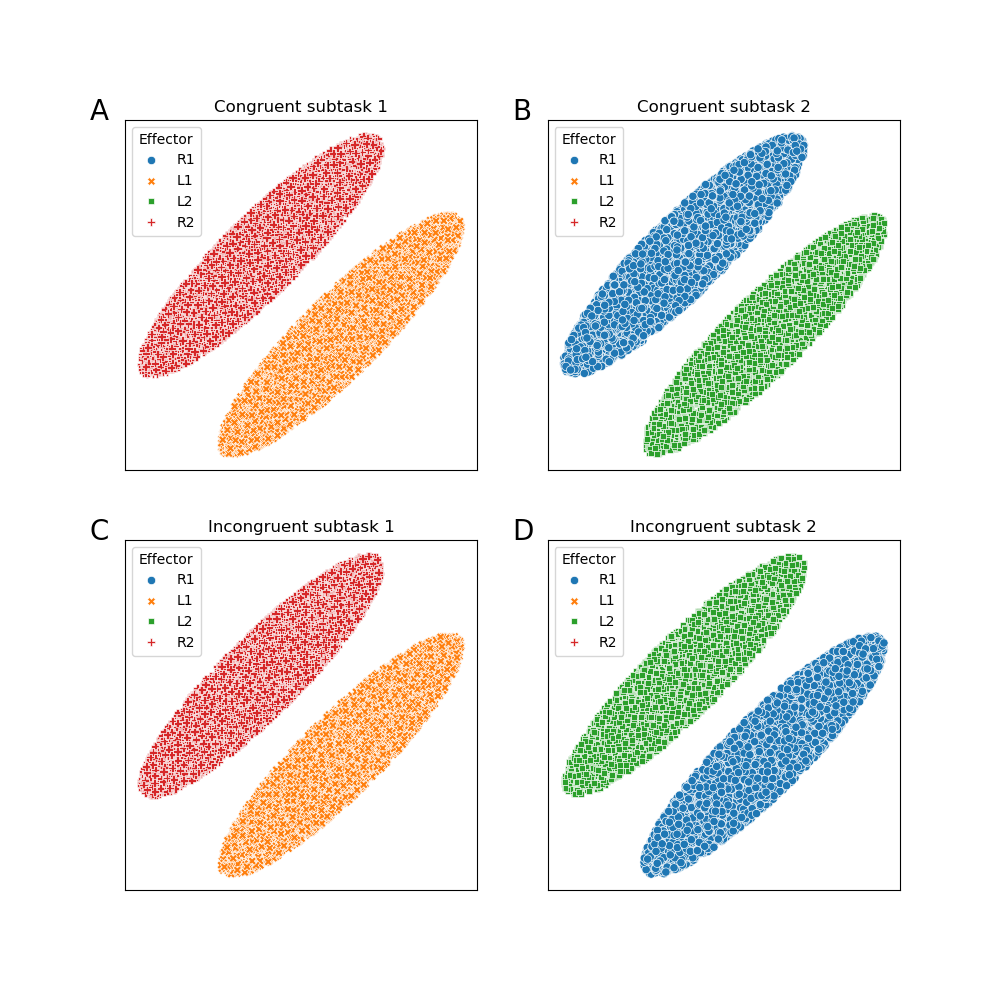
\includegraphics[width=0.7\textwidth]{../figures/fig_categories_stim_space.png}
    \caption{
        \textbf{A:} Stimulus distributions  and response assignments in the Congruent condition.
        \textbf{B:} Stimulus distributions  and response assignments in the Inongruent condition.
        In all panels, the colour of the points indicates the effector (and thus the response key) associated with the correct response.  R1 indicates the right index finger, R2 the right middle finger, L1 the left index finger, and L2 the left middle finger. Note that in Incongruent condition, stimuli from the same region of stimulus space are assigned to different
hands in different subtasks.}
    \label{fig:Cats}
\end{figure}

Note that if motor effectors are learned, there should be no difference between the Congruent and Incongruent conditions because in both cases, a unique effector is used to respond to all four categories. In contrast, if motor goals are learned then we would expect better performance in the Congruent Condition. First, note that in both conditions, four different effector mappings must be learned. So the conditions do not differ at this level.  However, note that only two motor goals need to be learned in the Congruent condition, whereas the Incongruent condition requires learning four motor goals. To see this, note that the stimuli in the upper left categories of the Congruent condition all have the motor goal ``press the button on the right'' in both subtasks. In contrast, in the Incongruent condition, these same stimuli have different motor goals in the two subtasks. 

\section{Methods}

\subsection{Design}
The stimuli in both II tasks were circular sine-wave gratings that varied across trials in their spatial frequency and their orientation. Gratings in the first
task were presented on a gray square background on top of a black screen, whereas gratings in the second task were
presented on a gray diamond background on top of a black screen. See Figure~\ref{fig_example_trials.png} for
examples.

\begin{figure}[h!]
    \centering
    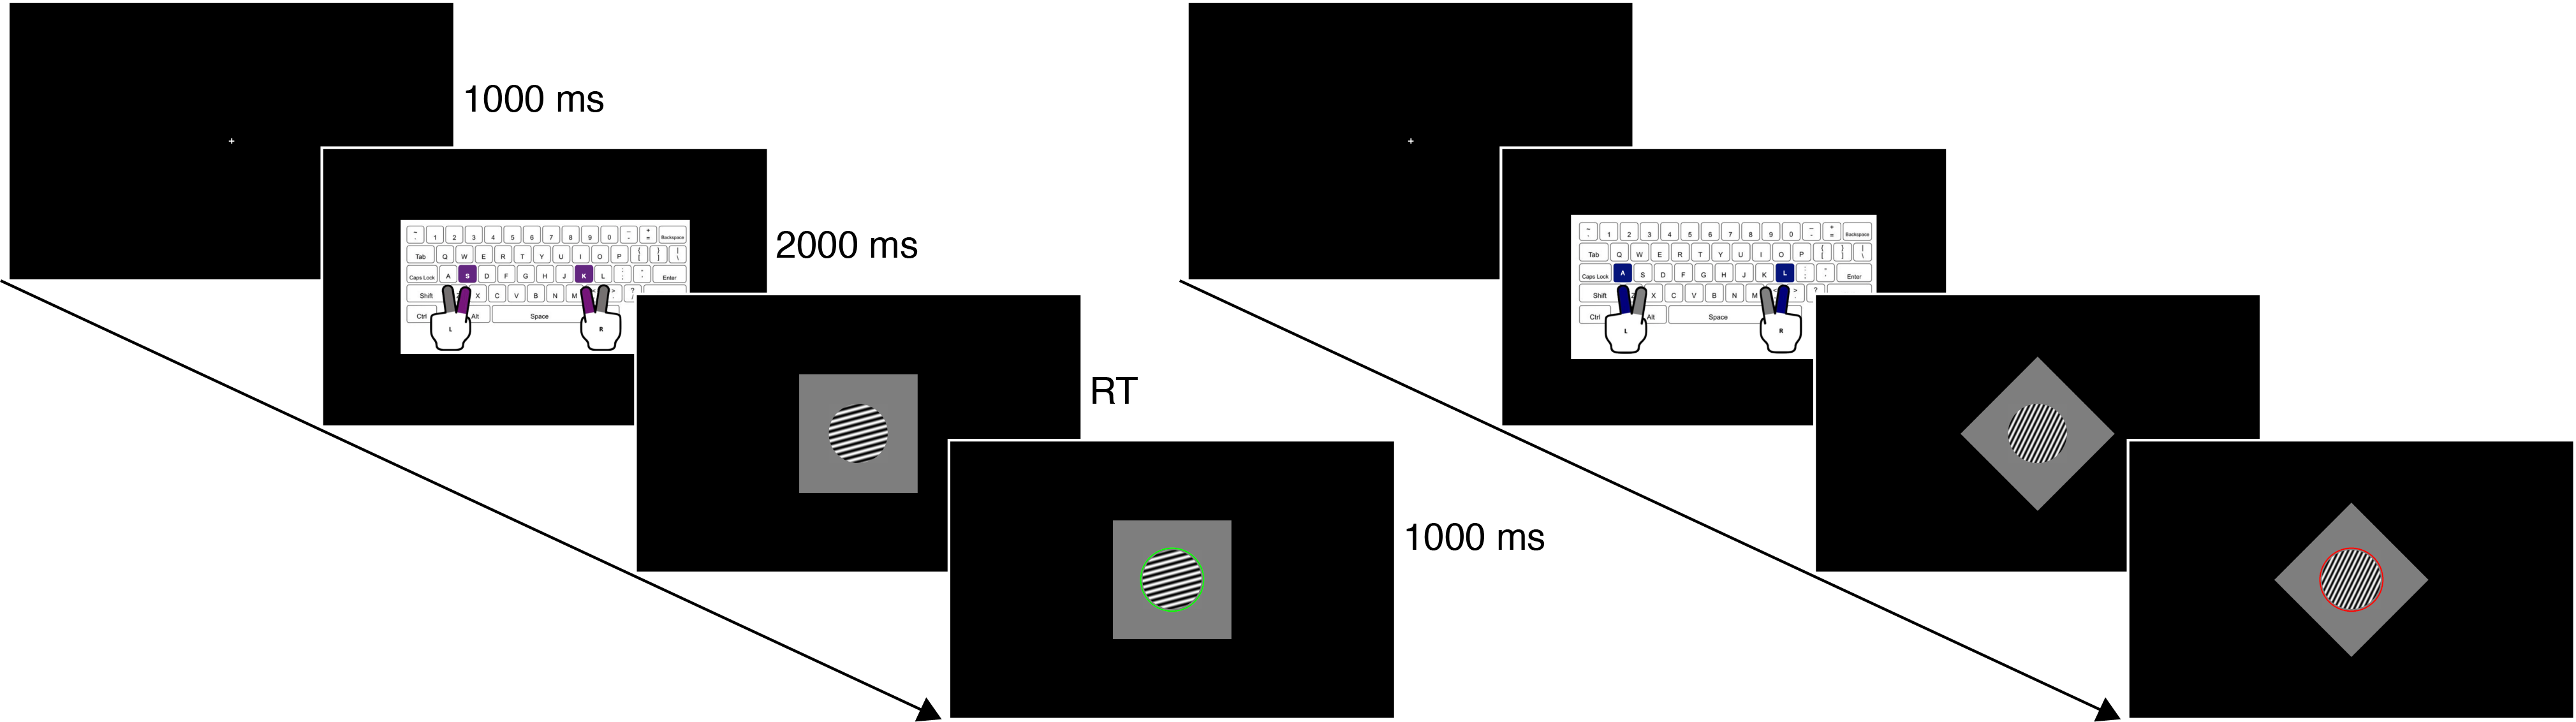
\includegraphics[width=\textwidth]{../figures/fig_example_trials.png}
    \caption{
    \textbf{Left:} Example Square subtask trial in which a
    correct response was given.  \textbf{Right:} Example
    Diamond subtask trial in which an incorrect response was
    given.
}
    \label{fig_example_trials.png}
\end{figure}

Participants were randomly assigned to one of two conditions -- Congruent or Incongruent. In the Congruent condition, stimuli from the same regions of stimulus space were assigned to fingers on the same hand in the two tasks. In contrast, in the Incongruent condition, participants used the same response keys as in the Congruent condition, but stimuli from the same regions of stimulus space were assigned to fingers on different hands in the two tasks. Please see Figure~\ref{fig:Cats} for a description of the exact mappings used.

\subsection{Participants}
The experiment included 91 participants.   One participant was excluded from the analysis for failing to
follow the instructions regarding which fingers and keys to
use to indicate category responses. The remaining 90
participants were either first-year undergraduate psychology
students from Macquarie University recruited via the Sona
system ($n = 28$) or individuals from the general community
($n = 62$), recruited via direct invitation from the
researchers. All Macquarie University undergraduate
participants completed the study and received course credit
for their participation.  All other participants volunteered
with no compensation. All participants were between 18 to 30
years of age, fluent in English, had normal or
corrected-to-normal vision and hearing and no history of
neurological impairments. Each participant was randomly
assigned to one of 2 conditions (Congruent and
Incongruent).  The 45 Incongruent participants included 12 males and 31 females. Their ages ranged from 18 to 27
years old ($M = 19.6$, $SD = 1.7$).  The 45 Congruent participants included 16 males and 29 females. Their ages
ranged from 18 to 30 years old ($M = 22.5$, $SD = 2.3$).  

\subsection{Stimuli and Categories}
The stimuli were circular sine-wave gratings that varied in
spatial frequency and orientation.  The coordinates of all stimuli were
generated by first sampling points in polar coordinates and
then converting them into Cartesian coordinates.
Specifically, radius values $r$ were sampled from a
uniform distribution on the interval $[0, 1]$, and angle
values $\theta$ were sampled uniformly from the interval $[0, 2\pi]$.
These polar coordinates $(r, \theta)$ were then transformed
into Cartesian coordinates $(x, y)$ using the equations $x =
r \cos(\theta)$ and $y = r\sin(\theta)$. This resulted in a
set of $(x, y)$ coordinates uniformly distributed within a
circle of radius 1 and centered at the origin. Next, $(x,y)$ coordinates were transformed from a circular uniform
distribution to an elliptical uniform distribution with horizontal major axis by multiplying the $x$ values by 124.02 and the $y$ values by 28.44. Finally, the
resulting coordinates were rotated by 45\degree and
translated by $(40, 60)$ for half the stimuli and by $(60,
40)$ for the other half. The resulting stimulus distributions
are shown in Figure~\ref{fig_2}.

\subsection{Procedure}
Participants provided informed consent form and were then given an optional
demographic questionnaire to complete. Participants were instructed that their task was to categorize circular sine-wave
gratings on the basis of their spatial frequency and orientation, and that each category was equally likely. They were also instructed that gratings presented on a square background may or may not require a different response policy than gratings presented on a diamond background. 

% TODO: check trial timing reported below
Each participant completed a single session consisting of
400 trials, with each task (square or diamond) interleaved
psuedo-randomly.   On each trial, participants viewed a
fixation cross (1000 ms), followed by a cue image that
indicated the correct finger-key mapping for the upcoming
task (2000 ms), followed by a response-terminated stimulus,
and then feedback (1000 ms).  Responses were given via the
``a'', ``s'', ``k'' and ``l'' keys as indicated by the cue
image (see Figure~\ref{fig:Cats}). Feedback
following correct responses was a green circle that appeared
around the stimulus, and feedback following incorrect
responses was a red circle. See
Figure~\ref{fig:Cats} an illustration of
example trials.

\subsection{Statistical Analysis}
We performed a logistic regression to examine the effects of condition (Congruent vs Incongruent), best-fitting decision-bound model (rule-based vs procedural), and log trial number on accuracy. All categorical predictors (i.e., condition and best-fitting decision-bound model) were dummy coded. Log trial number was used rather than trial number to account for the fact that the learning apparent in
Figure~\ref{fig_learning_curves} is non-linear, with more rapid initial improvements followed by slowed improvements as the task progressed. To assess whether there were differences in the proportion of participants best fit by a rule-based or procedural decision-bound model in each condition, we conducted a $\chi^2$ test. To assess switch costs, we computed the difference in accuracy and RT between
switch trials and stay trials for all trials across the
entire experiment for each participant. We then conducted a
2 (condition) $\times$ 2 (best-fitting decision-bound model) ANOVA
on the resulting switch costs.

\subsection{Decision-Bound Analysis}
To identify the decision strategy used by each participant,
we fit decision-bound models
\parencite{AshbyValentin2018} to
the trial-by-trial response data from the final 100 trials
of the experiment, separately for each participant and each subtask. We examined
1-dimensional rule-based models and 2-dimensional procedural
models.  The rule-based models assumed participants established a criterion on a single stimulus dimension and
then categorized stimuli based on whether or not they exceeded this criterion. These models had two free parameters -- a response criterion on the attended stimulus dimension, and the variance of perceptual and criterial noise. The 2-dimensional procedural models --
i.e., general linear classifier (GLC) --  assumed that participants used a linear decision boundary with an arbitrary slope and intercept to divide the stimulus space into two response regions. The GLC assumes that stimuli are categorized based on their position relative to this boundary. The GLC has three free parameters -- a slope and intercept of the decision bound and the variance of perceptual and criterial noise. For details on the models and the model-fitting process, see \textcite{AshbyValentin2018}.

\section{Results}

\subsection{Learning Curves}
Figure~\ref{fig_learning_curves}A shows the mean accuracy per block averaged over all participants for each condition.
The semi-transparent lines show performance separately for
each subtask and the solid lines show performance averaged
over both subtasks.  This figure clearly indicates that
learning proceeded more quickly and to a larger extent in
the Congruent condition than in the Incongruent condition.
Figure~\ref{fig_learning_curves}B shows the results for
participants best fit by a rule-based decision-bound model
and Figure~\ref{fig_learning_curves}C shows the results for
participants best fit by a procedural decision-bound model
(see the ``Decision Bound Models'' section for details). The
trend in both of these panels is the same as that observed
when considering all participants regardless of best-fitting
model (Figure~\ref{fig_learning_curves}A).

\begin{figure}[h!]
    \centering
    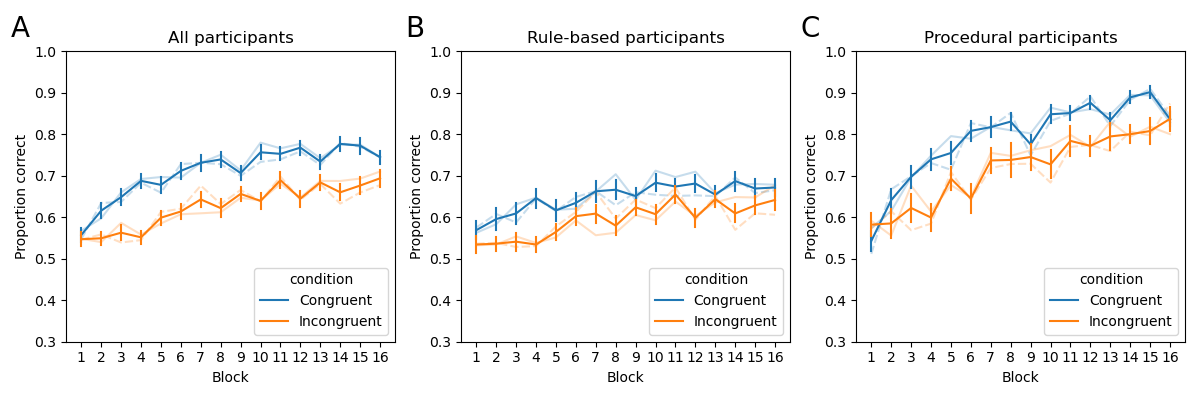
\includegraphics[width=1\textwidth]{../figures/fig_accuracy_per_block_by_model.png}
    \caption{
        \textbf{A:} Mean accuracy per block averaged over
        all participants. \textbf{B:} Mean accuracy per block
        averaged over participants best fit by a
        rule-based decision-bound model.  \textbf{C:} Mean
        accuracy per block averaged over participants
        best fit by a procedural decision-bound model.
        In all panels, blue lines correspond to the
        Congruent condition and orange lines correspond to
        the Incongruent condition.  The semi-transparent
        lines show the performance in each subtask, and the
        solid lines show the performance averaged over both
        subtasks. Error bars are standard errors of the
        mean.
    }
    \label{fig_learning_curves}
\end{figure}

We conducted a logistic regression to examine the effects of experimental condition (Congruent vs.  Incongruent),
decision-bound model (DBM: rule-based vs.  procedural), and their interactions on accuracy.  The results are summarized
in Table \ref{tab_logistic_regression}.  See the ``Statistical Analysis'' section for details. 
%
The effect of $\log(\text{trial})$ was significant [$\beta =
0.4775$, SE = 0.026, $z = 18.211$, $p < .001$], indicating
that accuracy increased across trials.  
%
The effect of Condition was not statistically significant [$\beta = 0.2289$, SE = 0.205, $z = 1.119$, $p = .263$], indicating that overall accuracy in the Congruent and Incongruent conditions was similar. 
%
However, the interaction between Condition and $\log(\text{trial})$ was significant [$\beta = -0.1321$, SE = 0.041, $z = -3.205$, $p = .001$], indicating that accuracy improved across trials more rapidly for the Congruent condition than in the Incongruent condition.
%
The three-way interaction of Condition, best-fitting decision-bound, and $\log(\text{trial})$ was also
significant [$\beta = 0.1361$, SE = 0.050, $z = 2.735$, $p = .006$], indicating that the rate of improvement in accuracy
across trials was greater in the Congruent condition than in the Incongruent condition, but only for participants best fit by a procedural model.
%
Overall accuracy was also significantly greater for
participants best fit by a procedural model than for
participants best fit by a rule-based model [$\beta =
0.9020$, SE = 0.167, $z = 5.386$, $p < .001$].
%
Participants best fit by a procedural model also showed a
greater improvement in accuracy across trials than
participants best fit by a rule-based model [$\beta =
-0.3348$, SE = 0.034, $z = -9.937$, $p < .001$].
%
The interaction between Condition and best fitting
decision-bound model was not significant [$\beta = -0.4712$,
SE = 0.249, $z = -1.895$, $p = .058$].

\begin{table}
\begin{center}
\caption{Logistic regression results. Condition is dummy
    coded with the Incongruent condition as the reference.
    Decidion-bound model (DBM) is dummy coded with the
    rule-based model as the reference.
}
\label{tab_logistic_regression}
\begin{tabular}{lcccccc}
  & \textbf{coef} & \textbf{std err} & \textbf{z} & \textbf{P$> |$z$|$} & \textbf{[0.025} & \textbf{0.975]}  \\
\midrule
\textbf{Intercept}                            &      -1.0034  &        0.129     &    -7.796  &         0.000        &       -1.256    &       -0.751     \\
\textbf{Condition}                            &       0.2289  &        0.205     &     1.119  &         0.263        &       -0.172    &        0.630     \\
\textbf{DBM}                                  &       0.9020  &        0.167     &     5.386  &         0.000        &        0.574    &        1.230     \\
\textbf{Condition:DBM}                        &      -0.4712  &        0.249     &    -1.895  &         0.058        &       -0.959    &        0.016     \\
\textbf{log(trial)}                           &       0.4775  &        0.026     &    18.211  &         0.000        &        0.426    &        0.529     \\
\textbf{condition:log(trial)}                 &      -0.1321  &        0.041     &    -3.205  &         0.001        &       -0.213    &       -0.051     \\
\textbf{DBM:log(trial)}                       &      -0.3348  &        0.034     &    -9.937  &         0.000        &       -0.401    &       -0.269     \\
\textbf{Condition:DBM:log(trial)}             &       0.1361  &        0.050     &     2.735  &         0.006        &        0.039    &        0.234     \\
\bottomrule
\end{tabular}
\end{center}
\end{table}

\subsection{Task Switching}
Figure~\ref{fig_switch_cost} shows switch costs for accuracy and RT for Congruent and Incongruent conditions for all participants, for participants best fit by a rule-based decision-bound model, and for participants best fit by a procedural decision-bound model. A 2 (condition) $times$ 2 (best-fitting decision-bound model) ANOVA revealed that the effect of
condition was significant [$F(1, 86) = 8.74, p < .001, \eta^2 = 0.09$], indicating that switch costs were greater
in the Incongruent condition than in the Congruent condition (see Figure \ref{fig_switch_cost}). However, the difference in switch cost between participants best fit by a procedural
model and participants best fit by a rule-based model was not significant [$F(1, 86) = 0.02, p = .88, \eta^2 = 0.00$]. The interaction term was also non-significant [$F(1, 86) = 0.01, p = .93, \eta^2 = 0.00$]. 

\begin{figure}[h!]
    \centering
    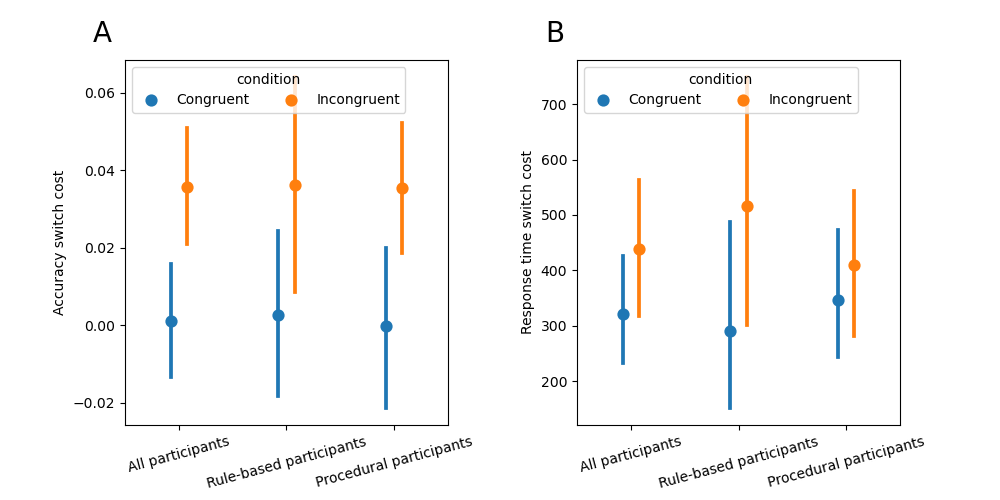
\includegraphics[width=1\textwidth]{../figures/fig_switch_cost.png}
    \caption{
        Accuracy switch costs (panel A) and RT switch costs (panel B) for both Congruent (blue) and Incongruent       (orange) conditions for all participants, for participants best fit by a rule-based decision-bound model, and for participants best fit by a procedural decision-bound model.
    }
    \label{fig_switch_cost}
\end{figure}

\subsection{Decision Bound Models}
Panels A, B, D, and E of Figure~\ref{fig_dbm} show the
decision bounds from the best-fitting decision-bound models
in both conditions overlaid on the underlying category
distribution for each subtask.  Figures~\ref{fig_dbm}C and \ref{fig_dbm}F show the proportion of participants whose responses were best fit by each type of model in each condition. For this analysis, we coded each particpant as a
procedrual model user if they were best by a GLC model on both subtasks, or as a rule-based model user if they were
best fit by an RB model on either subtask. This figure clearly shows that there were more procedural users in the
Congruent condition than in the Incongruent condition.  The results of Pearson's Chi-Squared test revealed that there were signifcantly more participants whose responses were best fit by a procedural model in the Congruent condition than in the Incongruent
condition [$\chi^2(1, N) = 200) = 4.48, p = .034, \text{Cramer’s} \, V = 0.16$].

\begin{figure}[h!]
    \centering
    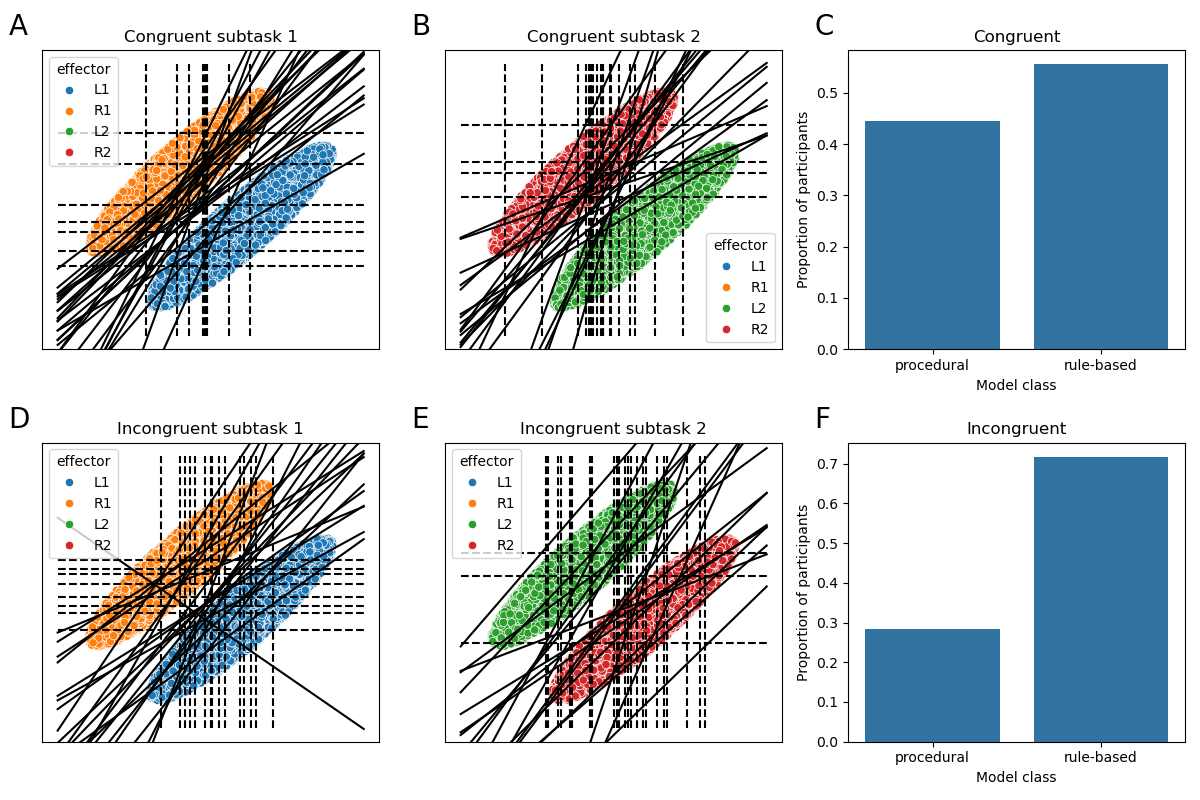
\includegraphics[width=0.9\textwidth]{../figures/fig_dbm.png}
    \caption{
        Category structures, best-fitting decision bounds, and decision-bound modeling results for each participant and subtask in each condition during the final 100 trials of training. 
  Row A) Results from the Congruent condition. 
  Row B) Results from the Incongruent condition.}
    \label{fig_dbm}
\end{figure}

\section{Discussion}
Procedural category learning is characterized by the gradual formation of many-to-one stimulus-response (SR) associations through trial-and-error feedback. Previous research in single-task
contexts suggests that these associations are linked to motor goals (e.g., pressing a button on the left) rather than specific motor effectors (e.g., pressing a button with a particular finger). The current study aimed to extend this finding to more ecologically valid conditions that included frequent task switching. Our goal was to investigate whether SR associations remain goal-based or shift to a more cost-effective effector-specific representation under these more complex and realistic conditions. For example, shifting to an effector-learning strategy could possibly offset the extra task-switching costs that are absent in almost all (single-task) laboratory studies of category learning. To investigate this question, participants learned two category structures while switching between tasks from the start of training, with motor responses varying across tasks. Our results showed more
effective learning when stimuli from the same region of stimulus space were mapped to responses on the same hand (Congruent condition), compared to when different hands were used (Incongruent condition).

An obvious first question when interpreting these results is to ask whether participants actually treated our task as an exercise in task switching, or rather as a single category-learning task with four categories. In this latter scenario, participants would have treated the context cue as a third stimulus dimension (with two values -- square or diamond; see Figure \ref{fig_example_trials.png}). Fortunately, this hypothesis is easy to rule out. First, we know that participants did attend to the context cue because accuracy was well over 50\% correct. Given that they attended to this cue, if they had treated it as a stimulus feature then there should be no switch costs, since there would be no task switching. In contrast to this prediction, our data showed clear switch costs in both conditions, which strongly suggests that participants in both conditions did treat the two subtasks as separate, and therefore did engage in frequent task switching. 

Given that participants did treat the two subtasks as separate, an important next question is to ask how strongly the tasks were separated. One possibility is that the tasks were separated perfectly, enabling participants to form independent, context-specific SR associations. Under this scenario, the learning of the two subtasks would proceed exactly as if each subtask was learned in isolation -- that is, under single task conditions. Each subtask  required learning SR associations that had two associated motor goals that required two separate motor effectors, and as a result, if participants had successfully formed independent SR associations for each task, we would expect no difference in learning performance between the Congruent and Incongruent conditions. Each task would have been learned in isolation, with no interference or generalization across contexts. However, this hypothesis is inconsistent with the significant difference in learning outcomes that we observed between the two conditions.  

An alternative view is that participants did form separate SR associations for each task but these associations were subject to some degree of generalization or interference across contexts. This view hypothesizes that participants learned a hierarchical representation of the two tasks. The context cue signaled which set of SR associations to activate on each trial and the two sets of SR associations were learned in the most efficient manner possible. This view makes different predictions depending on whether the SR learning was at the level of motor effectors or motor goals. If motor effectors were learned, there should have been no difference between the Congruent and Incongruent conditions because in both cases, a unique effector is used to respond to all four categories. In this case, a hierarchical representation does not simplify the problem. In contrast, if motor goals are learned then we would expect better performance in the Congruent Condition because the motor goal was the same in both subtasks. A hierarchical representation therefore simplifies motor-goal learning. As a result, the superior performance in the Congruent condition suggests that procedural category learning continues to rely primarily on motor goal-based SR associations during task switching. 

A more subtle interpretation of motor-effector learning is more difficult to rule out. Specifically, a more subtle hypothesis is that learning was at the effector level,  and performance was better in the Congruent condition because of generalization between effector representations. To see this, consider first the Congruent condition. After some learning, this hypothesis predicts that a subtask 1 stimulus from the upper-left category (see Figure \ref{fig:Cats}) will activate motor representations associated with movements of the right middle finger (i.e., R2 in Figure \ref{fig:Cats}). If these representations are broadly tuned, then activation will extend to neighboring motor regions. In fact, finger representations in primary motor cortex (i.e., in M1) are both somatotopic and widely overlapping for neighboring fingers \parencite{DechentFrahm2003, EjazEtAl2015}.  Therefore, activation of right middle finger representations are likely to also activate (albeit more weakly) right index finger representations (i.e., R1 in Figure \ref{fig:Cats}), which could in this way facilitate learning in subtask 2. 

Although our results can not conclusively reject this more subtle view of motor-effector learning, there are several reasons why we believe this alternative view is unlikely. First, note that this hypothesis predicts worse performance in the Incongruent condition only if activation of an effector representation on one hand activates the effector representations of neighboring fingers on the same hand significantly more than it activates the mirrored finger on the opposite hand.\footnote{For example, note that the upper-left categories in Figure \ref{fig:Cats} are associated with the right middle and index fingers in the Congruent condition and the right and left middle fingers in the Incongruent condition.} Although we know of no data that speaks conclusively to this issue, there is compelling evidence that finger movements on one hand activate motor representations of the mirrored finger on the other hand. For example,  \textcite{DiedrichsenEtAl2013} concluded that ``during unimanual ipsilateral finger presses, primary sensory and motor cortices show, underneath global suppression, finger-specific activity patterns that are nearly identical to those elicited by contralateral mirror-symmetric action'' (p. 1362).

Second, \textcite{ashby_procedural_2003} reported that single-task II categorization performance was unaffected when participants were suddenly required to switch hands on the response keys and begin key pressing with the mirrored finger on the opposite hand from training. In contrast, a number of studies have reported that switching the locations of the response keys significantly impairs II performance \parencite{ashby_procedural_2003, CrossleyEtAl2012, MaddoxBohilIng2004, MaddoxEtAl2007, SpieringAshby2008}.\footnote{Specifically, \textcite{ashby_procedural_2003} reported that switching to the mirrored finger caused an immediate, small drop in accuracy that quickly recovered to pre-switch levels. In contrast, switching the locations of the response keys caused a much larger drop in performance that never recovered.} Thus, both the available neural and behavioral data suggest that motor-effector learning should strongly generalize to the mirror finger on the opposite hand. This seems problematic for the subtle effector-learning hypothesis because it seems to predict little or no performance difference between the Congruent and Incongruent conditions. Future research could clarify this issue by including conditions with subtasks that vary the similarity of the effectors assigned to the same stimuli.

% 23. Dechent P, Frahm J. Functional somatotopy of finger
% representations in human primary motor cortex. Hum Brain
% Mapp 2003; 18:272–83. PMID: 12632465
% 
% 24. Ejaz N, Hamada M, Diedrichsen J. Hand use predicts the
% structure of representations in sensorimotor cortex. Nat
% Neurosci 2015;18.
% 
% 25. d’Avella A, Giese M, Ivanenko YP, Schack T, Flash T.
% Editorial: Modularity in motor control: from muscle
% synergies to cognitive action representation. Front Comput
% Neurosci 2015; 9:1–6.
% 
% 26. d’Avella A, Saltiel P, Bizzi E. Combinations of muscle
% synergies

\subsection{Relation to existing lines of research}
This study builds upon our previous investigation into the
effects of motor planning on task-switching in novel and
attention-demanding tasks \parencite{crossley_switch_2023,
crossley_trial-by-trial_2018, turner_hierarchical_2017}.  In
that earlier work, we were among the first to explore task
switching when the tasks are not only new to participants
but also challenging to learn.  One of the key findings was
that learning while task-switching was only possibly when
each task required unique motor responses.  The present study extends this line of inquiry by showing that the SR associations formed during task switching most likely remain at the level of motor goals. 

A line of studies from Collins and colleagues is also relevant to our current results \parencite{collins_cognitive_2013, collins_human_2014, collins_neural_2016, collins_motor_2016, collins_cost_2017}. In particular, \textcite{collins_motor_2016} showed that when task switching, humans prefer hierarchical rules in which
the motor responses used for a task are physically adjacent. However, the relevance of this result to our results is not clear since the Collins and Frank studies used much simpler tasks that included easily discernible stimuli and straightforward response rules. 

\subsection{Conclusions}
In summary, we believe that the most parsimonious interpretation of our results is that during more ecologically valid task-switching conditions, procedural category learning remains at the level of motor goals. This is somewhat surprising since effector learning is more computationally efficient. If the effector is learned, no further computation is needed to produce a response. In contrast, if a motor goal is learned, then extra computation is required to select an effector to accomplish this goal. One might expect that the extra cost of task switching would induce participants to switch to a more computationally efficient effector-learning strategy. Our results suggest this did not happen.

One reason that people might persist with the more computationally expensive motor-goal strategy is that it has much greater adaptive value. In natural environments, procedural learning is often used to learn motor actions that allow retrieval of some novel reward. If the learning is of motor goals then future experience can be used to sculpt and refine the motor actions to improve performance. However, if learning is at the effector level then the motor actions used during initial learning might become quicker with practice, but altering them in any substantive way will be problematic.

\subsection{Authors' contributions}
MJC wrote the paper, designed the experiments, performed all data analysis and modelling, and and oversaw data collection;
HA wrote the paper and collected all data.
DMK wrote the paper and oversaw data collection;
FGA wrote the paper and designed the experiments.

\printbibliography

\end{document}
